\chapter{Theory and Background}
In this chapter, I will provide the theoretical background necessary to understand the work presented in this thesis. The first section will deal with the definition and importance of the bandgap of a material, the second will introduce the effects of confinement on electrons within semiconductors, leading to a discussion of experimental confinement within the semiconductor quantum well. The third section will introduce the concept of semiconductor quantum well disorder, and the fourth will motivate the study of semiconductor quantum well disorder with micro photoluminescence spectroscopy. Finally, I will discuss the optical properties of asymetric double quantum wells and how to use photoluminescence excitation spectroscopy to investigate incoherent coupling between excitons in the asymmetric double quantum wells.

\section{The Semiconductor Quantum Well}
This section will broadly lay out band theory of electron states in solids. I will then discuss interband absorption by electrons in direct-gap semiconductors. 
\subsection{Bandgap}

%bandgap def, a little discussion
\indent In order to understand how electrons behave in a crystalline solid, one must first understand how bound electrons act when arbitrarily many atoms are brought together in a lattice structure. Consider a collection of $N$ atoms sufficiently far apart such that interactions between atoms can be neglected. In this limit, electrons in an atom such as Hydrogen occupy discreet energy levels. For instance: suppose all $N$ of our atoms are monatomic hydrogen atoms. In our system, an electron behaves according to the following Hamiltonian:
\begin{equation}
\hat{H} = -\frac{\hbar^2}{2m} \bigtriangledown^2 - \frac{e^2}{2\pi \epsilon_0 r}.
\end{equation}
We can find the electron wavefunctions $\psi(x)$ by solving the time independent Shr\"{o}dinger equation,
\begin{equation}
\hat{H}\psi(x) = E_n\psi(x)
\end{equation}
where $E_n$ is the energy of the $n^{th}$ energy level. This equation can be solved using the usual methods \cite{griffiths}, but doing so here would be a diversion, so I'll just skip to the crucial points: evidently, the $n=2$ electron wavefunction (again neglecting interactions between atoms and ground state perturbations) is
\begin{equation}
\psi(x) = Y^m_l\frac{1}{\sqrt{2}}a^{-3/2}_0\Big(1-\frac{r}{2a_0}\Big ) exp\big(-r/2a_0 \big)
\end{equation}
where $a_0$ is the Bohr radius, $Y^m_l$ is either the $l=0, m=0$, the $l=1, m=1$, or the $l=1, m=1$ spherical harmonic. Note: each $n = 2$ energy level in this system is $N$-fold degenerate, as there are $N$ orbitals with the same energy. Considering just the $n = 2$ states and neglecting perturbations, electrons in these states evidently all have energy
\begin{equation}
E_2 = \frac{-13.6eV}{n^2} = \frac{-13.6eV}{4}.
\end{equation}
In the limit that many atoms are brought together such that interactions can no longer be neglected, two things happen: each $N$-fold degenerate electron energy level will split into $N$ components, and these levels will become so close that they will smear into allowed and disallowed energy densities of state \cite{iadonisi, sirdesh, griffiths, davies, fox}. Roughly speaking, the occupied states are known as the ``valance band'' states, and the unoccupied states are known as the ``conduction band states''. The energy difference between the valance band and conduction band is called the bandgap, and its importance will be illuminated momentarily. 

\indent These band states are simultaneous eigenstates of both the Hamiltonian and the crystal momentum \cite{davies, fox}. This means that bands can be easily depicted in k-space using dispersion curves. Dispersion curves map out allowed band energies in k-space, and their full functional shape is dependent on the types and arrangement of constituent atoms.  Solids can be broadly organized into three categories based upon the k-space arrangement of their electron bands. In metals, the conduction band energies are below the highest energy valence band states and thus some conduction band states are occupied. In insulators, the bandgap is relatively large (about 10eV) \cite{fox}. By contrast in semiconductors, the bandgap is roughly 1eV and can therefore be optically accessed. Sometimes, as in the case of GaAs crystals, a local valance band minima and conduction band maxima occur for the same value of $k$ in k-space. Semiconductors with this sort of bandstructure are known as direct-gap semiconductors. Around this value of k, electrons can absorb a photon with enough energy to undergo a direct transition from the valance band to the conduction band \cite{iadonisi, galanthesis}. This fact forms the basis of linear and nonlinear optical studies of semiconductor nanostructures \cite{stevereview}, photonic devices, and certain types of theoretical quantum information processing schemes.

\begin{figure}[h]
\centering
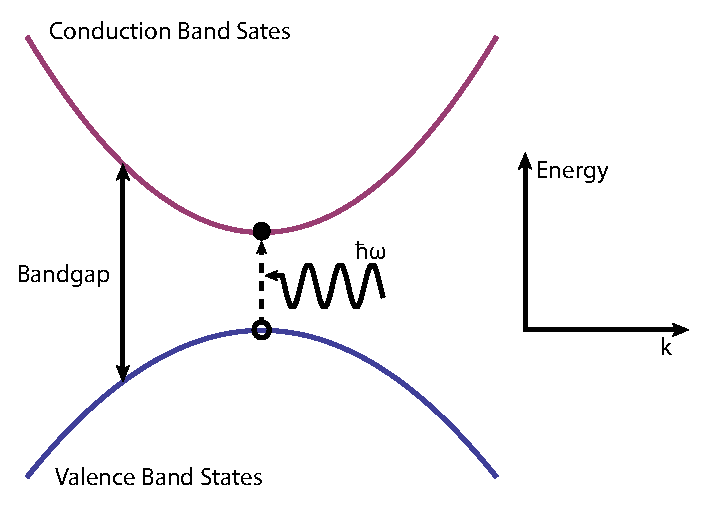
\includegraphics[width = .4\textwidth]{dispcurve.eps}
\caption{ \doublespacing A typical dispersion curve minima for a direct-gap semiconductor. An optical transition is illustrated at $k = 0$, where an electron is absorbing a photon resulting in a transition from the conduction band to the valance band.}
\label{ExampleBands}
\end{figure}

\begin{figure}[h!]
\centering
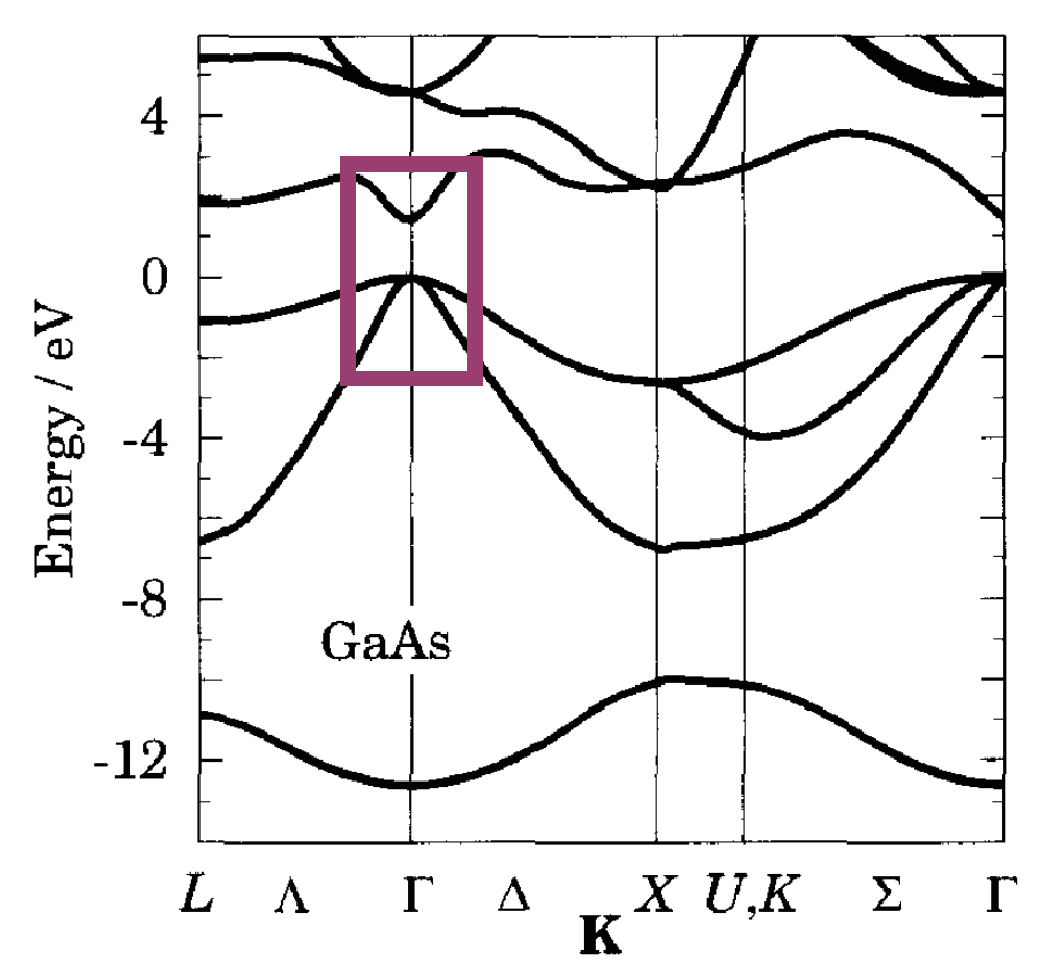
\includegraphics[width = .3\textwidth]{GaAsBstruct.eps}
\caption{\doublespacing The band structure of GaAs, the allowed states are the thick horizontal curves, and the boxed region is the direct-gap region, in which electrons can be make direct transitions across the bandgap. Note, the minima of this region look like the dispersion curve in figure 2.1 \cite{davies}.}
\label{GaAsBstruct}
\end{figure}
%dispersion curves


%Discussion of bands in GaAs and AlGaAs, p orbital smearing etc. Find p 63 in davies. (maybe here maybe later)
\newpage
\subsection{Confinement}
%confinement intro
\indent It is well known that nanometer scale confinement of particles results in quantized energy states \cite{griffiths}. In the previous section, I briefly introduced the bandgap, and its important physical properties. In this section, I'll illustrate an interesting application of band theory: the semiconductor quantum well (QW). First, it is important to understand what we mean by confinement, and how quantized energy levels arise for confined particles. I will draw an analogy to a familiar physical situation, the particle confined within an infinite potential. I will then use this analogy to construct a physical picture for QWs, and then I will discuss the formation of excitons and a simple physical model of their behavior, sufficient for understanding the spectroscopy conducted in this thesis.

\indent Perhaps the simplest problem in quantum mechanics is the of confinement of a particle in an infinite, one dimensional potential well. I will sketch a derivation of the wave function of a particle trapped in such a well, and use this derivation as the basis for exploring the physics of the QW exciton. We will begin by considering an arbitrary particle confined in a one dimensional infinite potential well. The potential that our arbitrary particle feels is:

\[ V(x) = \begin{cases} 
      0 & 0 < x < L \\
      \infty & |x| > 0 
   \end{cases}
\]
where $L$ is the length of the potential well. Graphically, the potential the particle feels looks like \ref{infp}.

\begin{figure}[h!]
\label{infp}
\centering
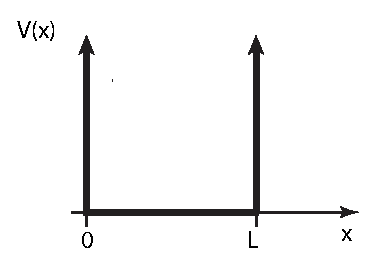
\includegraphics[width = .6\textwidth]{infpotential.eps}
\caption{\doublespacing A graphical representation of the one-dimensional infinite potential well of width $L$.}
\end{figure}

Our task is to solve the time independent Schr\"{o}dinger equation to show how quantized bound states arise for one-dimensional confinement. The time independent Schr\"{o}dinger equation reads:

\begin{equation}
\hat{H} \psi(x) = E\psi(x)
\end{equation}
where E is the energy of the particle, and $\psi(x)$ is the particle's wavefunction. The particle will evidently be confined to the well, so our Hamiltonian inside the well is just

\begin{equation}
\hat{H} = - \frac{\hbar^2}{2m} \frac{\partial^2}{\partial x^2}
\label{hamil}
\end{equation}
where $m$ is the particle's mass, and $E$ is the particle's  total energy. The time independent Schr\"{o}dinger equation now reads:

\begin{equation} \label{tise}
\frac{\partial^2}{\partial x^2} \psi(x) = - \alpha \psi(x)
\end{equation}
where we define 
\begin{equation}
\alpha = \frac{2mE}{\hbar^2}.
\end{equation}
Now, eq. 2.7 looks like the familiar simple harmonic oscillator equation from classical mechanics. Because the wave function must be continuous at $x = L$ and $ x = 0$, i.e. it vanishes at those locations, and the potential is odd about the origin,  solutions to eq. 2.7 have the form:
\begin{equation} \label{soln1}
\psi(x) = A sin(k x) 
\end{equation}
where $k$ contains $E$ and is determined by our boundary conditions. Now we want $\psi(L)$ to vanish, but we can't have $A =0$, because that is the trivial solution to eq. 2.7. Therefore, because we want $\psi(L) = Asin(k L) = 0 $, we must have $ka = \pm n \pi$ where $n \in \mathbb{N}$. Now, we can absorb all of the negative combinations of $k L$ into our normalization constant, $A$, and we have, then, that 
\begin{equation}
k_n L = n \pi 
\end{equation}
where the subscript denotes the fact that we now have infinitely many, \textit{discreet} solutions to eq. 2.5. Evidently 
\begin{equation}
k_n = \frac{ n \pi}{L}
\end{equation}
and therefore
\begin{equation}
\psi(x) = A sin(\frac{n \pi x}{L}).
\end{equation}
Now, if we let $k_n = \alpha$ and solve for E, we obtain
\begin{equation}
E = \frac{n^2 \pi^2 \hbar^2}{2 m L^2}.
\end{equation}
It will do us no good to normalize the wavefunctions we found, as their use for our purposes is minimal. The important part is that confinement in one dimension resulted in our particle occupying \textit{discreet} energy levels whose energy depends on the size of the confinement potential. 

\indent Using layers of semiconductors, one can generate similar one-dimensional confinement effects for electrons. A simple way this can be done is by sandwiching a layer of low-bandgap semiconductor material in between two layers of higher bandgap materials \cite{davies}. One period of this structure is shown in figure 2.4. If the well material is a direct-gap semiconductor, then simple optical transitions (i.e. not mediated by phonons) across the bandgap can be made, as the transition illustrated in figure 2.1. Figure \ref{GaAsBstruct} is the band structure for GaAs, the chosen well material for the studies of growth disorder. Annotated on the figure is the direct-gap transition zone of interest. The potential well created by the semiconductor sandwich leads to quantization of electron states within the well layer \cite{miller, davies, stevereview}. We can access each of these states optically, making the QW a great testbed for exploring electron dynamics within a simple and well-known potential \cite{stevereview}. 




\begin{figure}[h!]
\centering
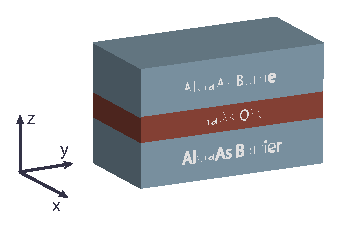
\includegraphics[width = .4\textwidth]{Well.eps}
\caption{\doublespacing An example of the semiconductor quantum well. These layers can be repeated arbitrarily many times.}
\label{GaAsBstruct}
\end{figure}

\newpage
\subsection{The Exciton}

\indent The simple picture presented above doesn't quite adequately represent the physics of an electron within a quantum well, however. After an excited electron moves from the valence band to the conduction band, it will leave behind a vacancy, or ``hole'', around its parent atom \cite{miller, davies}. The electron feels a \textit{screened} Coulomb potential from this vacancy, as the vacancy is positively charged. I'll briefly sketch why this potential arises and then introduce the key concept of this section: the exciton. Imagine a number of electrons have been excited within the QW. Now, spatially, one will have a quasi-neutral distribution of electrons and holes in the well layer: an electron-hole plasma. I will assume that the holes are stationary relative to the electrons in the well, and that the excitation density is relatively low. These assumptions are \textit{a priori} unphysical, but they immensely simplify the derivation of the electric potential QW electrons feel, and preserve the important physical results. 

\indent Let's explore the local behavior of an excited electron due to a single adjacent hole in the QW. Note that in this picture, electrons everywhere in the QW feel a Coulomb attraction to the hole, but the electrons adjacent to the hole screen its effects from charges far away. This phenomenon, known in plasma physics as Debye shielding \cite{chen} and in quantum mechanics as electron screening \cite{griffiths}, modifies the pure Coulomb potential one would expect a single electron-hole pair to experience. We will assume that the electrons in the plasma obey a Maxwellian density distribution. Now, the local density of electrons around the hole is 

\begin{equation}
n_e = n_{0}~ exp \Big[ \frac{e\phi}{k T}\Big]
\end{equation}
where $n_{0}$ is the electron density far away, $e$ is the electron charge, $\phi$ is the local electromagnetic potential, and  $T$ is the electron temperature. A complete derivation for this electron number density in an arbitrary plasma can be found in CITE Chen. This is the local electron distribution, and we can assume $e\phi \ll kT$ because the potential an electron feels due to one hole can be considered small relative to its thermal energy. Taylor expanding to first order, we find that
\begin{equation}
n_e \approx n_0 \Big[ \frac{e\phi}{k T}\Big ].
\end{equation}
Now, our local charge density is 
\begin{equation}
\rho(r) = e \Big [ \delta(r) - n_0 \Big( \frac{e\phi}{k T}\Big ) \Big]
\end{equation}
where we've assumed that the hole has positive charge magnitude $e$, is infinitely small, and situated at the origin. The Poisson equation reads
\begin{equation} \label{pois}
\epsilon_0 \bigtriangledown^2 \phi(r) = -e \Big [ \delta(r) + n_0 \Big( \frac{e\phi}{k T}\Big ) \Big].
\end{equation}
We can define a constant, 
\begin{equation}
k^2 = \frac{n_0 e\phi}{\epsilon_0 k T}
\end{equation}
and now the Poisson equation is
\begin{equation}
\big(\bigtriangledown^2 - k^2 \big) \phi = - \frac{e \delta(r)}{\epsilon_0}.
\end{equation}
This is known as the screened Poisson equation, and its solution is
\begin{equation}
\phi(r) = -\frac{e}{4\pi \epsilon_0 r} e^{-k r}.
\end{equation}
\indent Now, $\phi(r)$, functionally,  the correct result (albeit with a different k) had we proceeded under the Thomas-Fermi approximation, assuming only that the potential is weak and varies smoothly and slowly over a distance around the hole equivalent to $\frac{1}{k_f}$. This turns out to be a very good approximation for the local potential an electron feels relatively close to a hole CITE Patterson. The single-particle hamilltonian for an electron in the QW is now:
\begin{equation}
\hat{H} = - \frac{\hbar^2}{2m} \frac{\partial^2}{\partial x^2} - \frac{e}{4\pi \epsilon_0 r} e^{-k_0 r}
\end{equation}
where $k_0^2 = \frac{n_0 e\phi}{k T_f}$ is the ``corrected'' k for the same potential derived under the Thomas-Fermi approximation \cite{patterson}. 

\indent Note that if the potential electrons feel was exactly Coulombic in nature, then any bound state between an electron and a hole would be hydrogenic \cite{griffiths}. This potential, however, is \textit{not} exactly Culombic in nature, so the bound states between the electrons and holes can't be described by hydrogenic wavefunctions. Nevertheless, bound states between an exited electron and an adjacent hole do exist, and when an electron and hole occupy these states, they form a quasiparticle called an ``exciton", and they can be treated as a single particle with an effective mass \cite{iadonisi, davies}.

\indent The subtleties of the wave function are treated in \cite{iadonisi}, exploring their exact functional form and corresponding density of exciton states in the QW will not be of use to us here. Only energy levels of the QW exciton are discretized by its confinement, those of excitons created in the bulk are not. A final important note: in both my derivation and those proceeding under the Thomas-Fermi approximation, the hole is assumed to be a \textit{stationary} point particle. This is emphatically \textit{not} true, but the physics doesn't change that much if we assume both charge carriers are mobile. Excitons can still be treated as a single particle even removing this assumption. Figure 2.5 depicts a simple physical picture for excitons: the electron and hole excited energy levels can be thought of as the ground state of a particle trapped in a finite potential.  

\begin{figure}[h!]
\label{Spapprox}
\centering
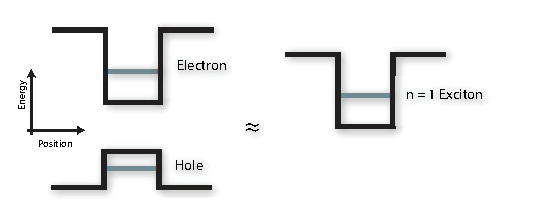
\includegraphics[width = .7\textwidth]{SpApprox.eps}
\caption{\doublespacing A simple model for the behavior of an exciton in a quantum well, suitable for the work completed herein.}
\label{GaAsBstruct}
\end{figure}


\section{Quantum Well Disorder}
\indent When an exciton is optically created, in a direct gap semiconductor such as GaAs, the charge carriers can recombine from the either exciton ``ground'' state ($n=1$), or ``excited''  states ($n>1$) and emit a photon at the exciton binding energy \cite{gilleo}. Since I am only interested in linear, long-timescale exciton physics, we can treat QW excitons as an approximately two-level system, only looking at ground state recombination. The emission energies for QW excitons will be dependent on well depth, a function of the barrier composition, and well width. Control of QW layer thickness has improved immensely, as QW structures can be made to precise specifications with modern molecular beam epitaxial growth methods \cite{davies}. However, imperfections of layer width on the order of a crystal monolayer occur unavoidably at the interface between the well and barrier materials during the QW manufacturing process \cite{yoshitaterrace} paper (find better). In figure 2.6, an AFM picture of imperfections of a GaAs surface are shown. These defects, known as structural disorder, slightly change the width of the well layer and thus subtly modulate exciton emission energies, an illustration of which is shown in figure 2.7. By analogy to eq. 2.11, excitons localized in slightly thinner than average sections of the QW will emit at slightly higher energies than average. Conversely, excitons localized in thicker than average sections of the QW will emit at slightly lower energies than average. Thus, structural disorder is the main contribution to inhomogeneous broadening in the QW coherent optical response \cite{bristowsep}. 

\begin{figure}[h!]
\label{disorder}
\centering
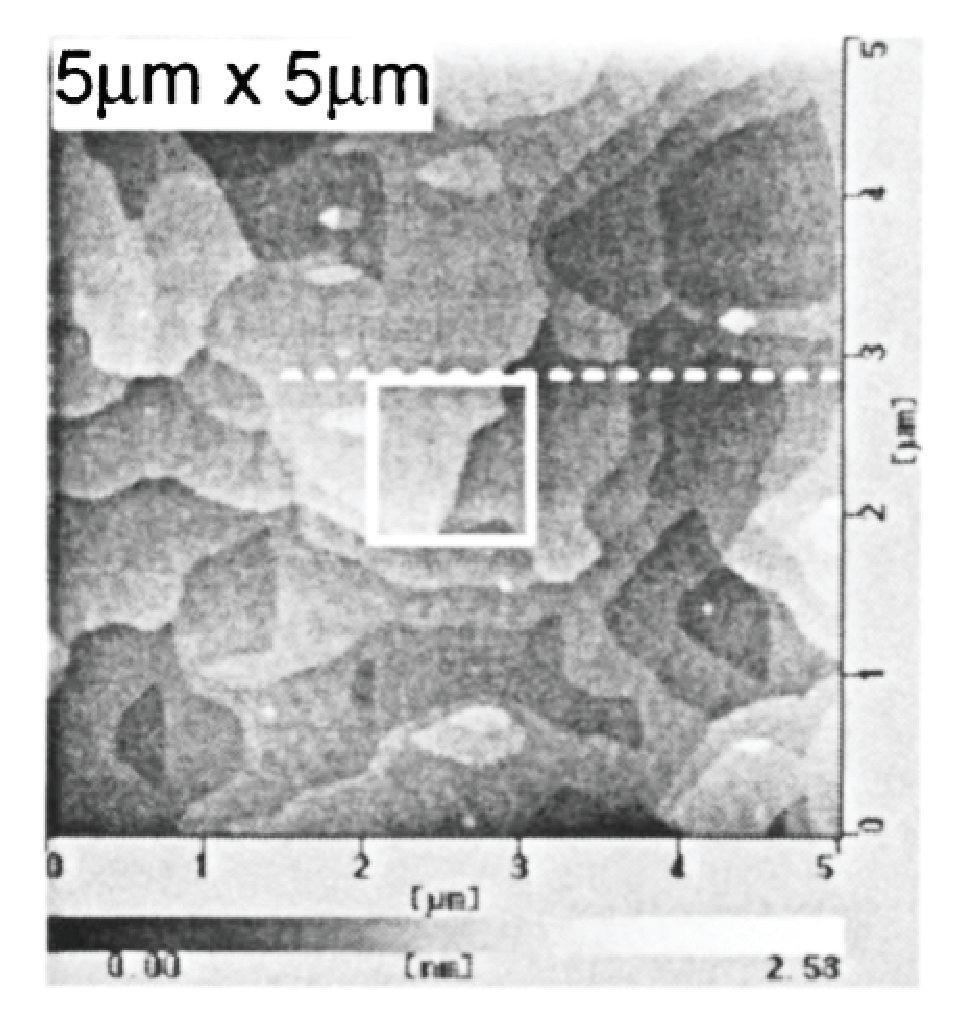
\includegraphics[width = .4\textwidth]{disorder.eps}
\caption{\doublespacing An STM picture of the GaAs growth front, stopped mid-growth, of a 110 oriented sample. The shown defect size is roughly representative of disorder in modern GaAs samples grown by molecular beam epitaxy. However, defect size and shape is highly sample dependent, so disorder varies widely from one QW structure to the next. Note, the disorder terraces are on the order of 100nm across. Adapted from \cite{yoshitaterrace}.}
\label{rel}
\end{figure}

\newpage
\begin{figure}[t!]
\label{rel-thickness}
\centering
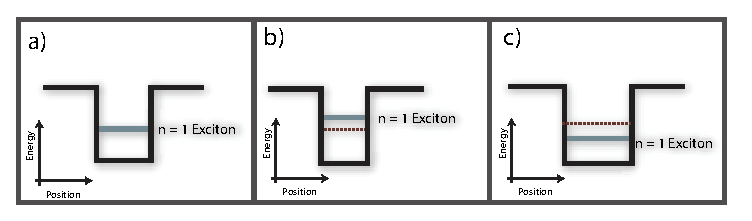
\includegraphics[width = .9\textwidth]{rel-thickness.eps}
\caption{\doublespacing In a), the energy of a ground state exciton located in a portion of the QW of average thickness, the blue line in b) depicts the ground state energy of an exciton located in a slightly thinner than average portion of the QW,  and in c), the blue line depicts the ground state energy of an exciton located in a slightly thicker than average portion of the QW. In both b) and c), the average exciton ground state energy is depicted by the maroon dashed line.}
\end{figure}

\section{Exciton Coupling in Asymmetric Double Quantum Wells}

\indent Quantum coupling between excitons occurs when multiple quantum wells get close enough so that the exciton wavefunction can tunnel slightly into adjacent wells \cite{griffiths, davies}. In order to study quantum coupling between states in adjacent QWs, however, it is not simply enough to grow multiple quantum well layers fairly close to one another. Evidently, if each of the wells is of identical thickness, then QW PL  from one well will be spectrally indistinguishable from another. Indeed, it is necessary to grow wells of varying thickness when studying coupling in multiple quantum wells \cite{hegartycouple}. 

\indent Asymmetric multiple quantum well (AQW) samples are a convenient system in which to study exciton coupling between wells. Incoherent coupling between exciton states, through temperature mediated CITE Borri T, dipole-dipole interactions  \cite{tomita}, or other incoherent processes can be quantified. Photoluminescence Excitation spectroscopy (PLE), a linear technique, can provide information on the energies and locations of various exciton states in AQWs. Coupling between wells is of interest because an improved understanding of the various processes that govern carrier transfer in nanostructures can help improve the efficiency and quality of nanostructure devices like photodiodes and transistors. Additionally, an increased understanding of exciton coupling processes is of fundamental research interest.



\section{Microphotoluminescence Spectroscopy}
\indent Because local QW thickness determines exciton emission energy, a spatial picture of disorder is possible through spectral imaging. By using a continuous wave (CW) excitation source to create a population of QW excitons and monitoring the emission energy as a function of sample position, one can extract the local QW width \cite{bristowsep}. With sufficiently high resolution, obtaining a map of emission energies for a representative portion of a QW sample is possible. In order to obtain a map of emission energies, one must monitor the photoluminescence (PL) energies as a function of position. In a PL experiment, light of sufficiently high energy is shown on a sample, exciting a large number of charge carriers to the conduction band. During this process, electrons fall back into holes in the valance band, emitting a photon equivalent to the lost energy \cite{davies}. If a QW exciton recombines, it will emit a photon equivalent the energy difference between the valance band and one of the quantized exciton states. If we regard the exciton as a two level system, by exciting QW excitons near-resonantly, the energy of the emitted photon will be equivalent to the energy difference between the valance band and the exciton ground state. 

\indent In order to obtain an image of PL, we must collect the signal carefully. More precisely, if we are to obtain a spatial picture of QW disorder, we must collect and spectrally resolve a PL image. The PL will be emitted from the exciton population over a $4 \pi$ solid angle, so we must place the QW directly at the focus of our imaging system in order to form a clear PL image. Furthermore, since the scale of the disorder is on the order of 100nm \cite{yoshitaterrace}, we must have comparable resolution for the PL image. Measuring a PL image is fairly easy, one must place the QW at the focus of a pair of lenses in a confocal optical geometry. Figure 2.8 is a diagram of this setup, and the magnification of the PL image is set by the ratio of the lens focal lengths. Namely,
\begin{equation}
M = \frac{f_1}{f_2}
\end{equation}
where $f_2$ and $f_1$ are the focal lengths of the short focal length lens and the long focal length lens respectively, and $M$ is the image magnification factor. A PL experiment with sub-micron resolution which is capable of spectrally resolving a PL image is known as a ``microphotoluminescence spectroscopy" experiment, or $\mu$PL.
\begin{figure}[h!]
\label{confocal}
\centering
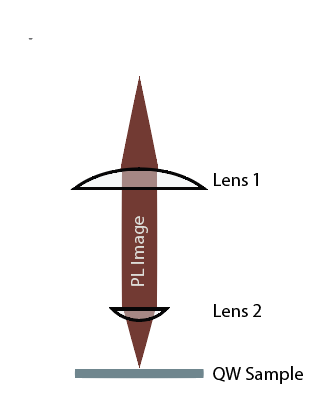
\includegraphics[width = .3\textwidth]{confocal1.png}
\caption{\doublespacing A representation of a confocal optical geometry used to collect the PL from the QW sample. The PL image is being collected from a small region of the QW sample, magnified, and then collimated by the two lenses.}
\end{figure}

\indent As simple as the PL image collection is, it is difficult to obtain the requisite image resolution because the PL is around 750-800nm wavelength, but as I've asserted above, the islands can be smaller than this. What this means is that if we were able to image at the Abbe diffraction limit of our optical geometry, we still wouldn't have the resolution necessary to resolve adjacent disorder sites. The Abbe diffraction limit is
\begin{equation}
d = \frac{\lambda}{2nNA}
\end{equation}
where $\lambda$ is the wavelength of the PL image, $n$ is the index of refraction in the intermediate space between the sample and lens 2 (the imaging lens) in figure 2.8, and $NA$ is the numerical aperture of lens 2. Note that $NA = f / D$ where $f$ is the focal length of the imaging lens and $D$ is its diameter. In our case, $d \approx 500 nm$ for $\lambda \approx 780 nm$, $n = 1$ in vacuum, and we pick $NA = .83$, as that was the NA of the lens in our experimental setup. 

\indent In order to get around this limit, we either need to resort to exotic microscopic techniques, or we can employ a fairly simple trick. It has been shown that by increasing the index of refraction ($n$) with a solid immersion lens (SIL), the Abbe diffraction limit can be substantially reduced  \cite{yoshitaapp} paper, and broad SIL paper. In order to do this, one simply places a hemisphere of sufficiently high $n$ material between the sample and the imaging lens. Figure 2.9 is a diagrammatic representation of this improvement. Note, I'll use SIL and hemisphere interchangeably from here on out, though they aren't necessarily interchangeable, as ``SIL'' refers to a truncated sphere of some degree. 

\indent In my experimental setup, I used a Zinc Selenide (ZnSe) SIL, for which $n = 2.4$ at $\lambda = 780 nm$. This improvement decreases the diffraction limit from $d \approx 500nm$ to $ d \approx 185 nm$, roughly sufficient resolution for our purposes. I'll expand on the precise setup in the next chapter, but the experiment will be very similar to what I've just described.
\begin{figure}[h!]
\label{confocal2}
\centering
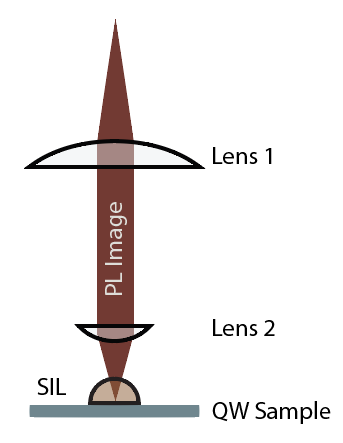
\includegraphics[width = .3\textwidth]{confocal2.png}
\caption{\doublespacing A representation of the principle of our specific $\mu$PL experiment. The PL image leaves the SIL normal to the hemispheric surface, so it just increases $n$ and lowers the diffraction limit.}
\end{figure}


\section{Photoluminescence Excitation Spectroscopy}
\indent I employ photoluminescence excitation (PLE) to study exciton coupling in AQW systems. PLE is a simpler method than $\mu$PL, as only the relative PL intensity is monitored. Generally, one looks at PL amplitude at a specific wavelength as the excitation wavelength is scanned across a wide range of wavelengths. By monitoring the PL as a function of excitation wavelength, one obtains a measure of absorption by the sample \cite{fox}. By extending this technique slightly, I can quantify the coupling between excitons in AQW samples. In order to do this, I scan the excitation wavelength of our light source, and take a PL spectrum (not just a single intensity value) for each different excitation wavelength. That way, the emission from both wells can be monitored as a function of excitation wavelength, and coupling between wells can be quantified: as the excitation wavelength scans over an exciton resonance in one well, the PL signal from the other well can be monitored to see if that resonant excitation increases emission.
